\section{Введение}

\subsection{Требования к ядру}
Рекомендуется использовать ядро Linux 4.9 (релиз в декабре 2016 года) или более
новое. Некоторые параметры конфигурации ядра должны быть включены.
Вот эти параметры: \\
\ci{CONFIG\_BPF=y}
\ci{CONFIG\_BPF\_SYSCALL=y}
\ci{CONFIG\_BPF\_JIT=y}
\ci{CONFIG\_HAVE\_EBPF\_JIT=y}
\ci{CONFIG\_BPF\_EVENTS=y}

\subsection{Схема BCC}
\url{https://github.com/iovisor/bcc}

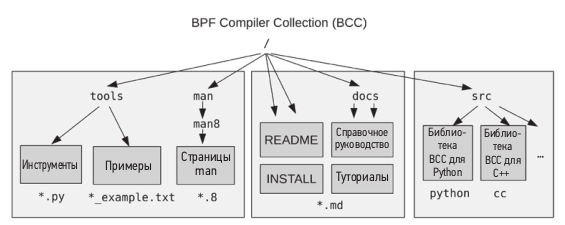
\includegraphics[width=0.8\linewidth]{structure_bcc.png}


\subsection{Установка в Ubuntu}
\cn{sudo apt-get update}
\cn{sudo apt-get install bpftrace}

\url{https://github.com/bpftrace/bpftrace}

\subsection{Схема bpftrace}
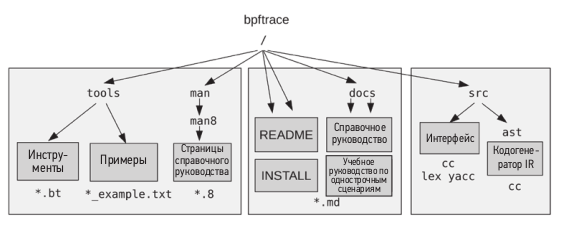
\includegraphics[width=1.0\linewidth]{structure_bpftrace.png}
